% \begin{frame}[t]
%   \frametitle{Perte de Huber}
%     {\footnotesize
%   \begin{align*}
%     L_{\text{Huber}} : \RR \times \RR & \rightarrow \RR \\
%     y, f(\xvec) & \mapsto 
%                   \begin{cases}
%                     \frac{1}{2} \left(y - f(\xvec)\right)^2 & \text{ si } |y - f(\xvec)| < \epsilon \\
%                     \epsilon |y - f(\xvec)| - \frac{1}{2} \epsilon^2 & \text{ sinon.} 
%                   \end{cases}
%   \end{align*}}
%    \begin{center}
%      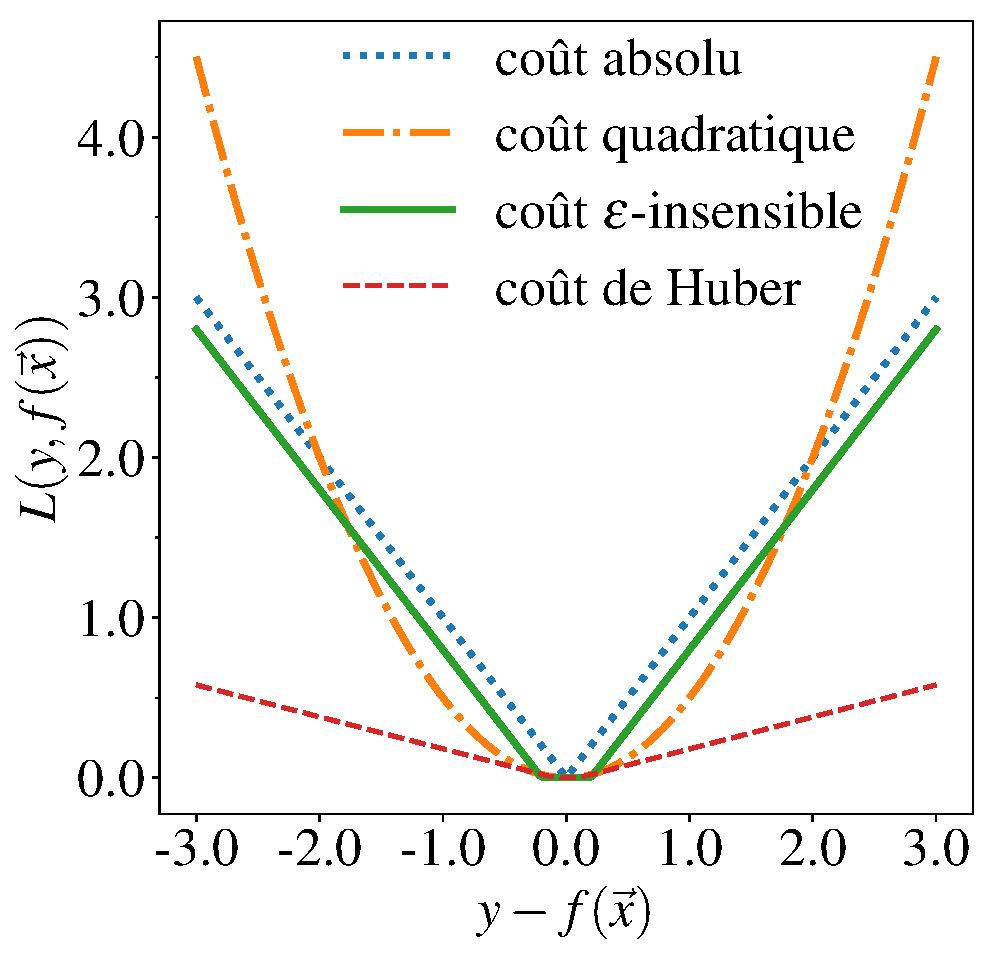
\includegraphics[width=0.5\textwidth]{figures/regression_losses}
%    \end{center}
%  \end{frame}


\begin{frame}
  \frametitle{Clustering ou partitionnement}
  \begin{itemize}
  \item \red{Clustering :} partitionner les données en sous-ensembles (\red{clusters}) homogènes
  \item Exemples :
    \begin{itemize}
    \item \blue{segmentation de marché}
    \item \blue{communautés} sur un réseau social
    \item \blue{topic modeling} (thématique de textes)
    \item \blue{compression} ou \blue{segmentation d'images}
    \item \blue{sous-types} d'une maladie
  \end{itemize}
  \end{itemize}
\end{frame}

\begin{frame}
  \frametitle{Clustering : Motivation}
  \begin{itemize}
  \item Étude de données \blue{non-étiquetées}
  \item Analyse \blue{exploratoire}
  \item \blue{Visualisation}
  \item Peut précéder une phase d'\blue{inférence}
  \end{itemize}
\end{frame}


\begin{frame}
  \begin{center}
    \large{1. Évaluation d'un clustering}
  \end{center}
\end{frame}

\begin{frame}
\frametitle{1.1 Critères géométriques}
  \begin{center}
    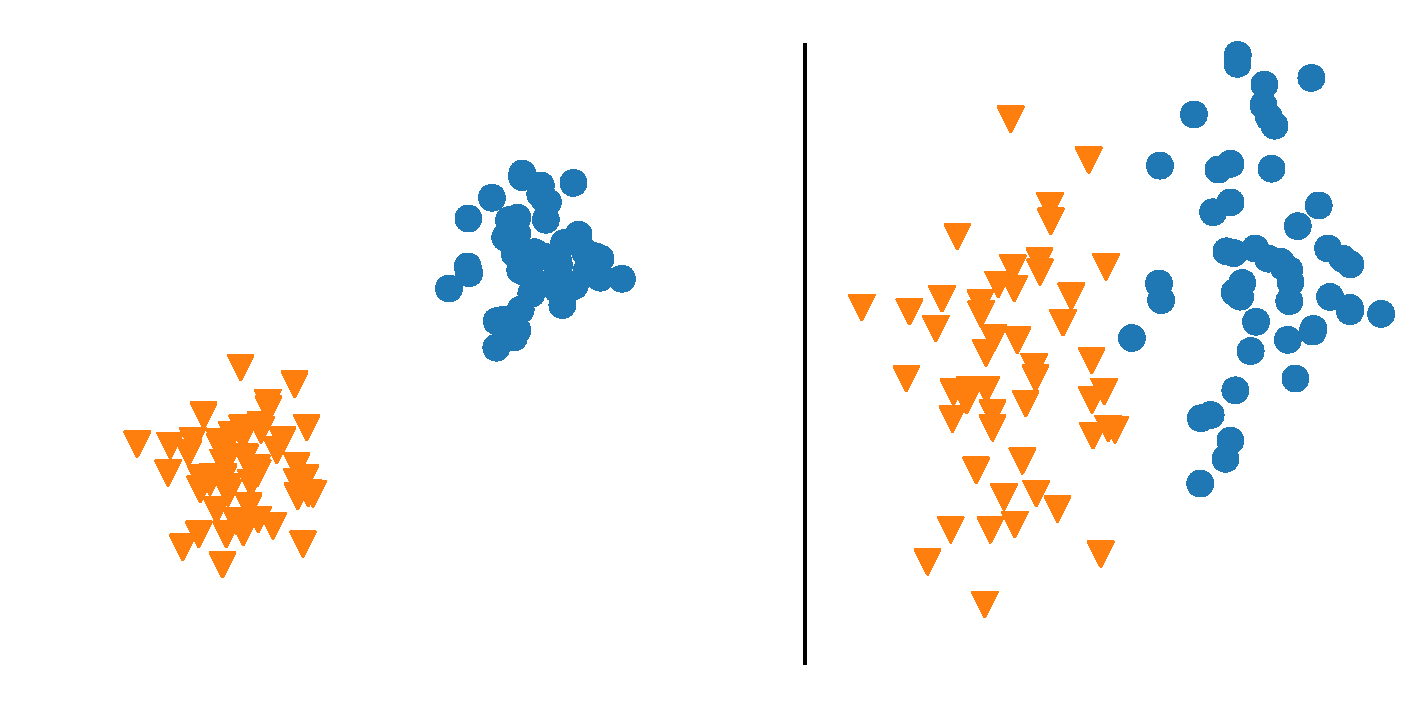
\includegraphics[width=0.5\textwidth]{figures/homogeneity}%
  \end{center}
\begin{itemize}  
  \item Définition centroïde du cluster $\cset$: $\muvec_{\cset} = \frac{1}{\cset}\sum_{\xvec \in \cset}\xvec$
  \item Définition médoïde du cluster $\cset$: $\mvec_{\cset} = \argmin_{\xvec \in \cset}d(\xvec, \muvec_{\cset})$
  \item \red{Dispersion} d'un cluster $k$ : $T_k = \frac{1}{|\cset_k|} \sum_{\xvec \in \cset_k} d(\xvec, \muvec_k)$
  % \begin{equation*}
  % T_k = \frac{1}{|\cset_k|} \sum_{\xvec \in \cset_k} d(\xvec, \muvec_k)
  % \end{equation*}
  \item Dispersion d'un clustering : 
  \begin{equation*}
  T = \frac1K\sum_{k=1}^{K}T_k
  \end{equation*}
\end{itemize}
\end{frame}

\begin{frame}
\frametitle{1.1 Critères géométriques}
  \begin{center}
    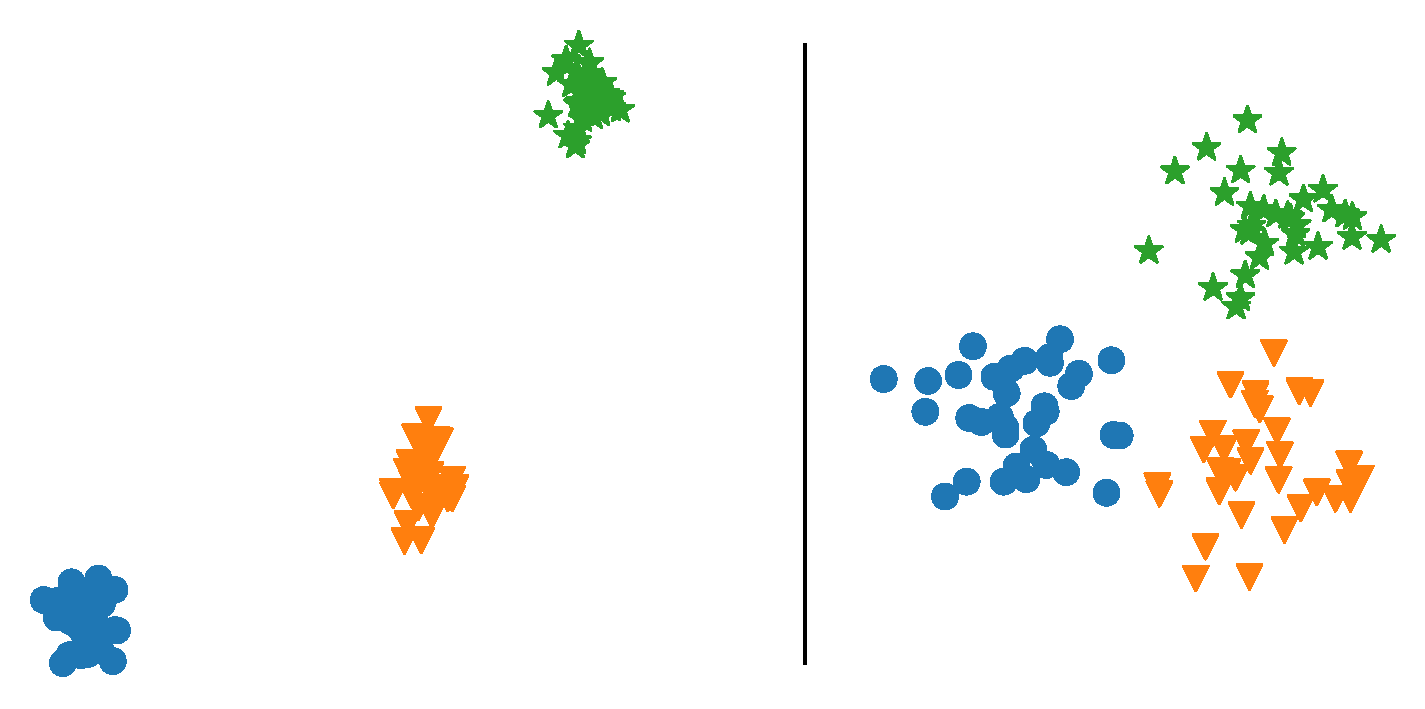
\includegraphics[width=0.5\textwidth]{figures/separability}%
  \end{center}
\begin{itemize}
  \item Séparabilité des clusters $k$ et $l$ : 
  \begin{equation*}
  s_{kl} = d(\muvec_k, \muvec_l)
  \end{equation*}
  \item Séparabilité d'un clustering : 
  \begin{equation*}
  S = \frac{2}{K(K-1)}\sum_{k=1}^{K-1}\sum_{l=k+1}^{K}s_{kl}
  \end{equation*}
\end{itemize}
\end{frame}


\begin{frame}
\frametitle{1.1 Critères géométriques}
\begin{itemize}
  \item  \textbf{Coefficient de silhouette.} On note d'abord $a(\xvec)$ la moyenne des distances entre $\xvec$ et les autres points du cluster $k(\xvec)$ auquel $\xvec$ est assigné :
  %\item Coefficient de silhouette. On note d'abord $a(\xvec)$ comme la moyenne des distances de $\xvec$ et des autres points dans le cluster $k(\xvec)$ auquel $\xvec$ est assigné.   
  \begin{equation*}
  a(\xvec) = \frac{1}{|\cset_{k(\xvec)}| - 1} \sum_{\uvec \in \cset_{k(\xvec)}}d(\xvec, \uvec)
  \end{equation*}
  \item La quantité $b(\xvec)$ est définie comme la plus petite valeur moyenne des distances entre $\xvec$ et tous les points d’un autre cluster $l \neq k(\xvec)$ :
%  \item La valeur $b(\xvec)$ correspond à la même expression, mais calculée pour le cluster autre que $k(\xvec)$, pour lequel la valeur est minimale:   
  \begin{equation*}
  b(\xvec) = \min_{l\neq k(\xvec)}\frac{1}{|\cset_l|} \sum_{u \in \cset_l}d(\uvec, \xvec)
  \end{equation*}
\end{itemize}
\end{frame}

\begin{frame}
  \frametitle{Coefficient de silhouette}
  \begin{center}
    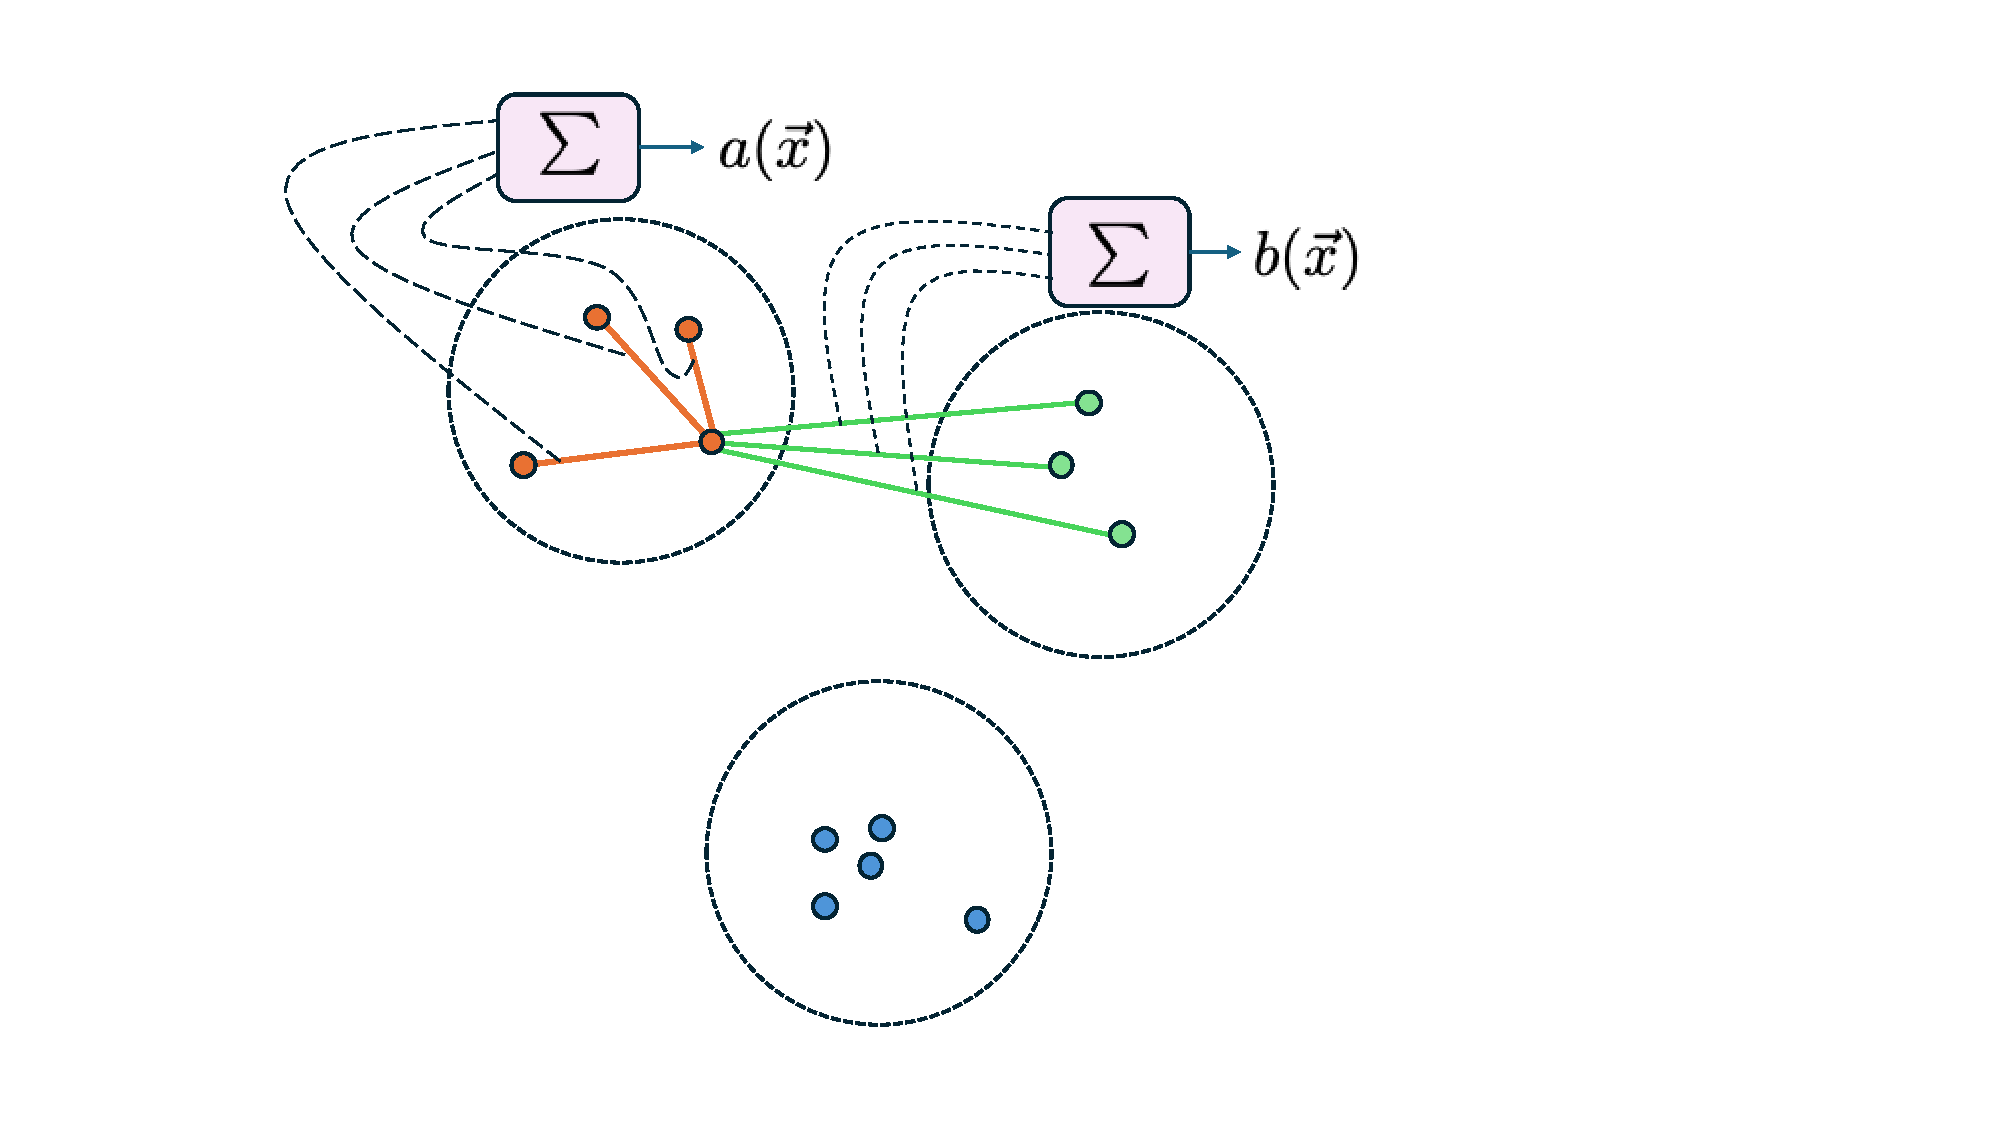
\includegraphics[width=0.9\textwidth]{figures/sillhouette_score}%
  \end{center}
\end{frame} 

\begin{frame}
\frametitle{1.1 Critères géométriques}
\begin{itemize}
  \item Avec $a$ et $b$ définis ainsi, nous pouvons définir le coefficient de silhouette pour le point $\xvec$ : 
  \begin{equation*}
  s(\xvec) = \frac{b(\xvec)-a(\xvec) }{\max{(b(\xvec), a(\xvec))}  }
  \end{equation*}
  \item Finalement, le \red{coefficient de silhouette} pour le clustering est :
  \begin{equation*}
  s = \frac1n \sum_{i=1}^{n}s(\xvec^i)
  \end{equation*}

\end{itemize}
\end{frame}

\begin{frame}
  \frametitle{1.2 Comparaison à des étiquettes connues}
  \begin{itemize}
  \item Difficulté : les clusters sont numérotés arbitrairement. 
  \pause
  \item \red{Indice de Rand} : pourcentage de paires de points qui sont soit dans le même cluster dans les deux partitions, soit dans des clusters différents dans les deux partitions : 
    \begin{equation*}
      \text{RI} = \frac2{n (n-1)} \sum_{i=1}^n \sum_{l=i+1}^n 
      \indic_{k(\xvec^i) = k(\xvec^l)} \, \indic_{y^i = y^l} + 
      \indic_{k(\xvec^i) \neq k(\xvec^l)} \, \indic_{y^i \neq y^l}.
    \end{equation*}

  \item Problème du RI : deux partitions aléatoires peuvent avoir un RI élevé par hasard. 
  \item Solution : ARI (adjusted Rand index) est le RI corrigé. 

  \end{itemize}
\end{frame}

\begin{frame}
  \frametitle{1.3 Stabilité des clusters}
  \begin{itemize}
    \item Génération de plusieurs partitions avec le même algorithme de clustering en variant : 
    \begin{itemize}
      \item les conditions initiales de l'algorithme
      \item des sous-échantillonages dans $\dset$
      \item des sous-ensembles de descripteurs (éventuellement)
    \end{itemize}
    \item On compare les résultats de clustering.
    \item Dans un clustering robuste, les résultats ne devraient pas varier trop. 
  \end{itemize}
\end{frame}


\begin{frame}
  \begin{center}
    \large{2. Clustering hiérarchique}
  \end{center}
\end{frame}

\begin{frame}
  \frametitle{Construction}
  \begin{itemize}
  \item Construction \red{agglomérative} \textcolor{gray!70}{(bottom-up)}
    \begin{itemize}
    \item Initialement : chaque point est son propre cluster 
    \item On fusionne itérativement les clusters les plus proches
    \end{itemize}
  \item Construction \red{divisive} \textcolor{gray!70}{(top-down)}
    \begin{itemize}
    \item Intialement : tous les points sont dans le même cluster 
    \item On sépare itérativement les clusters en deux
    \end{itemize}
  \end{itemize}
\end{frame}

\begin{frame}
  \frametitle{Clustering hiérarchique -- Principe}
  \begin{center}
    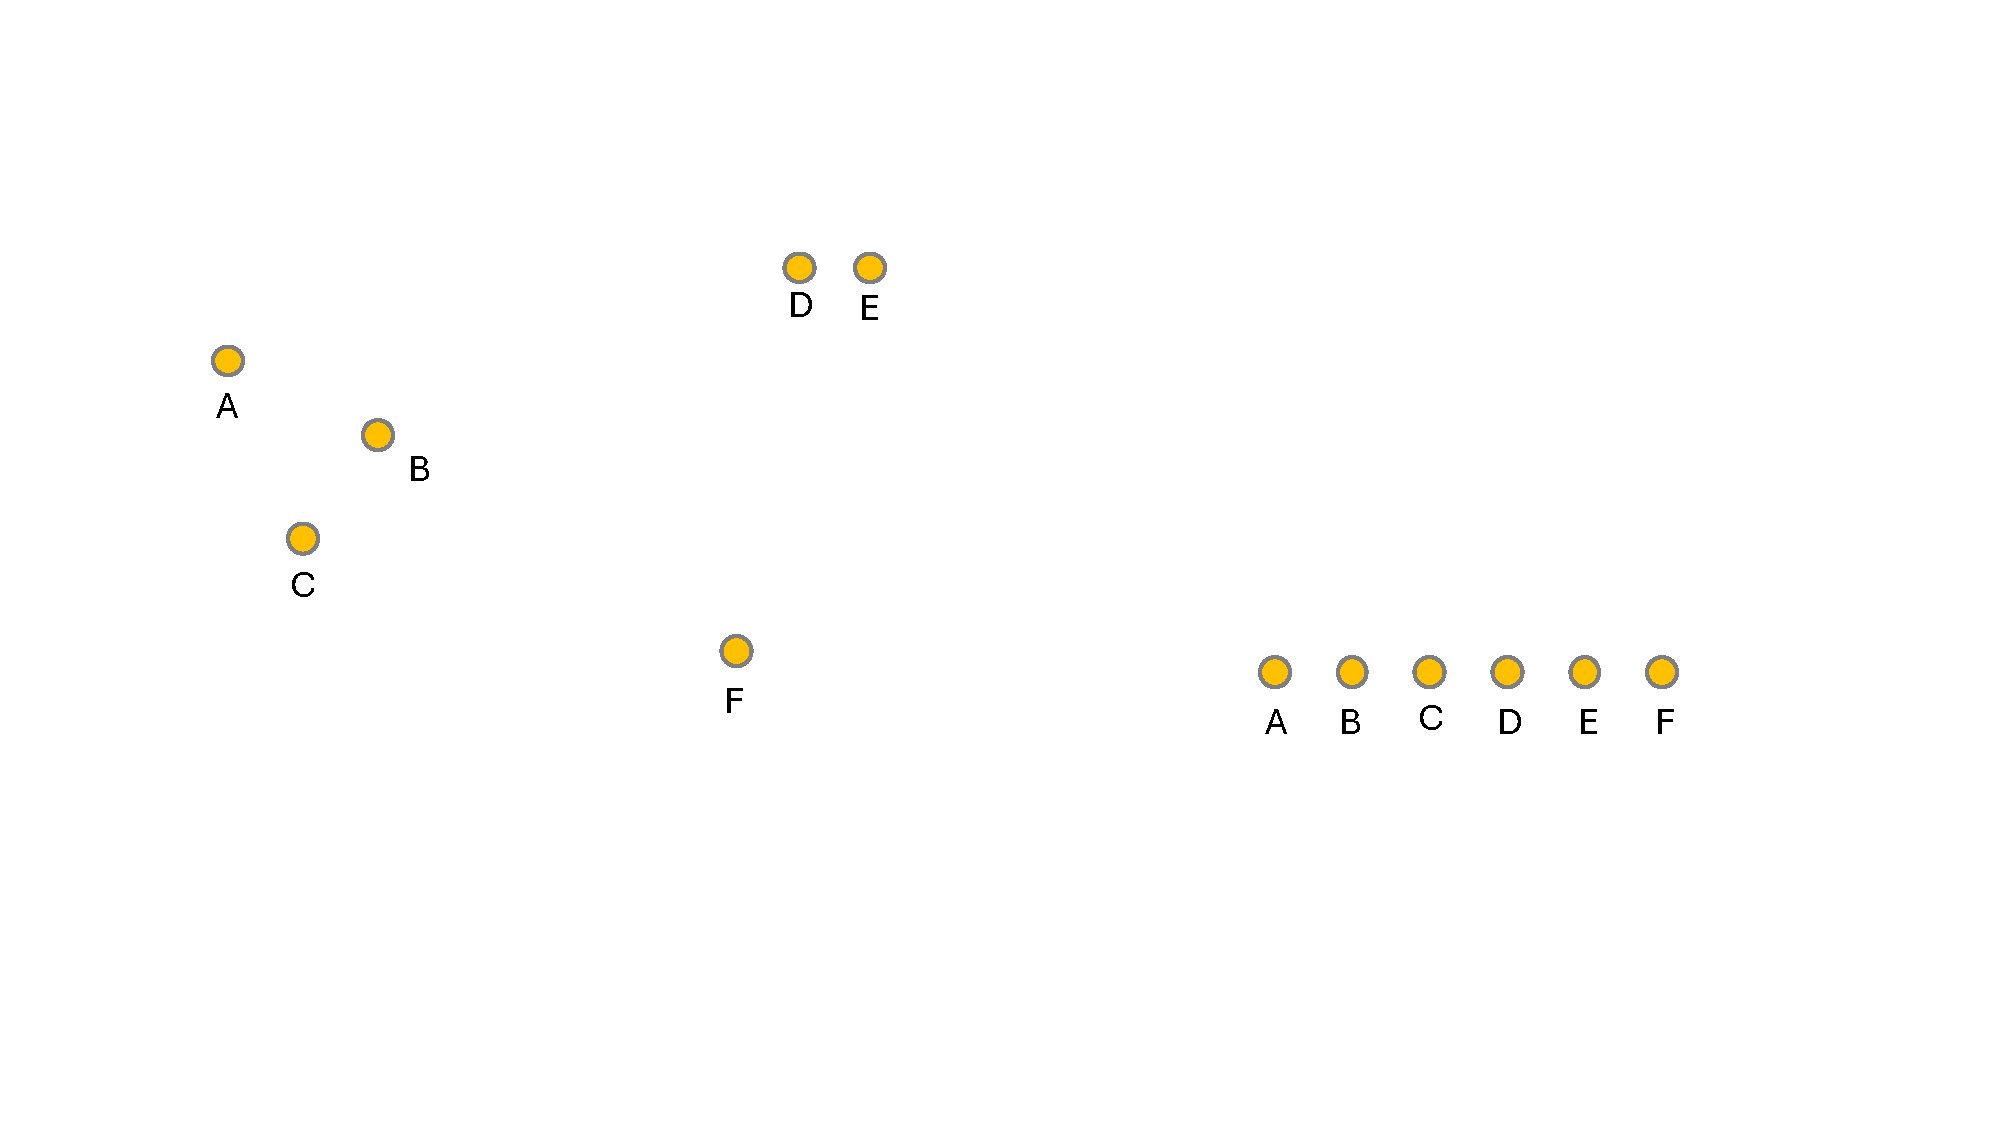
\includegraphics[width=0.8\textwidth]{figures/ch1}
  \end{center}
  Initialisation : chaque point constitue son propre cluster.
\end{frame}

\begin{frame}
  \frametitle{Clustering hiérarchique -- Principe}
  \begin{center}
    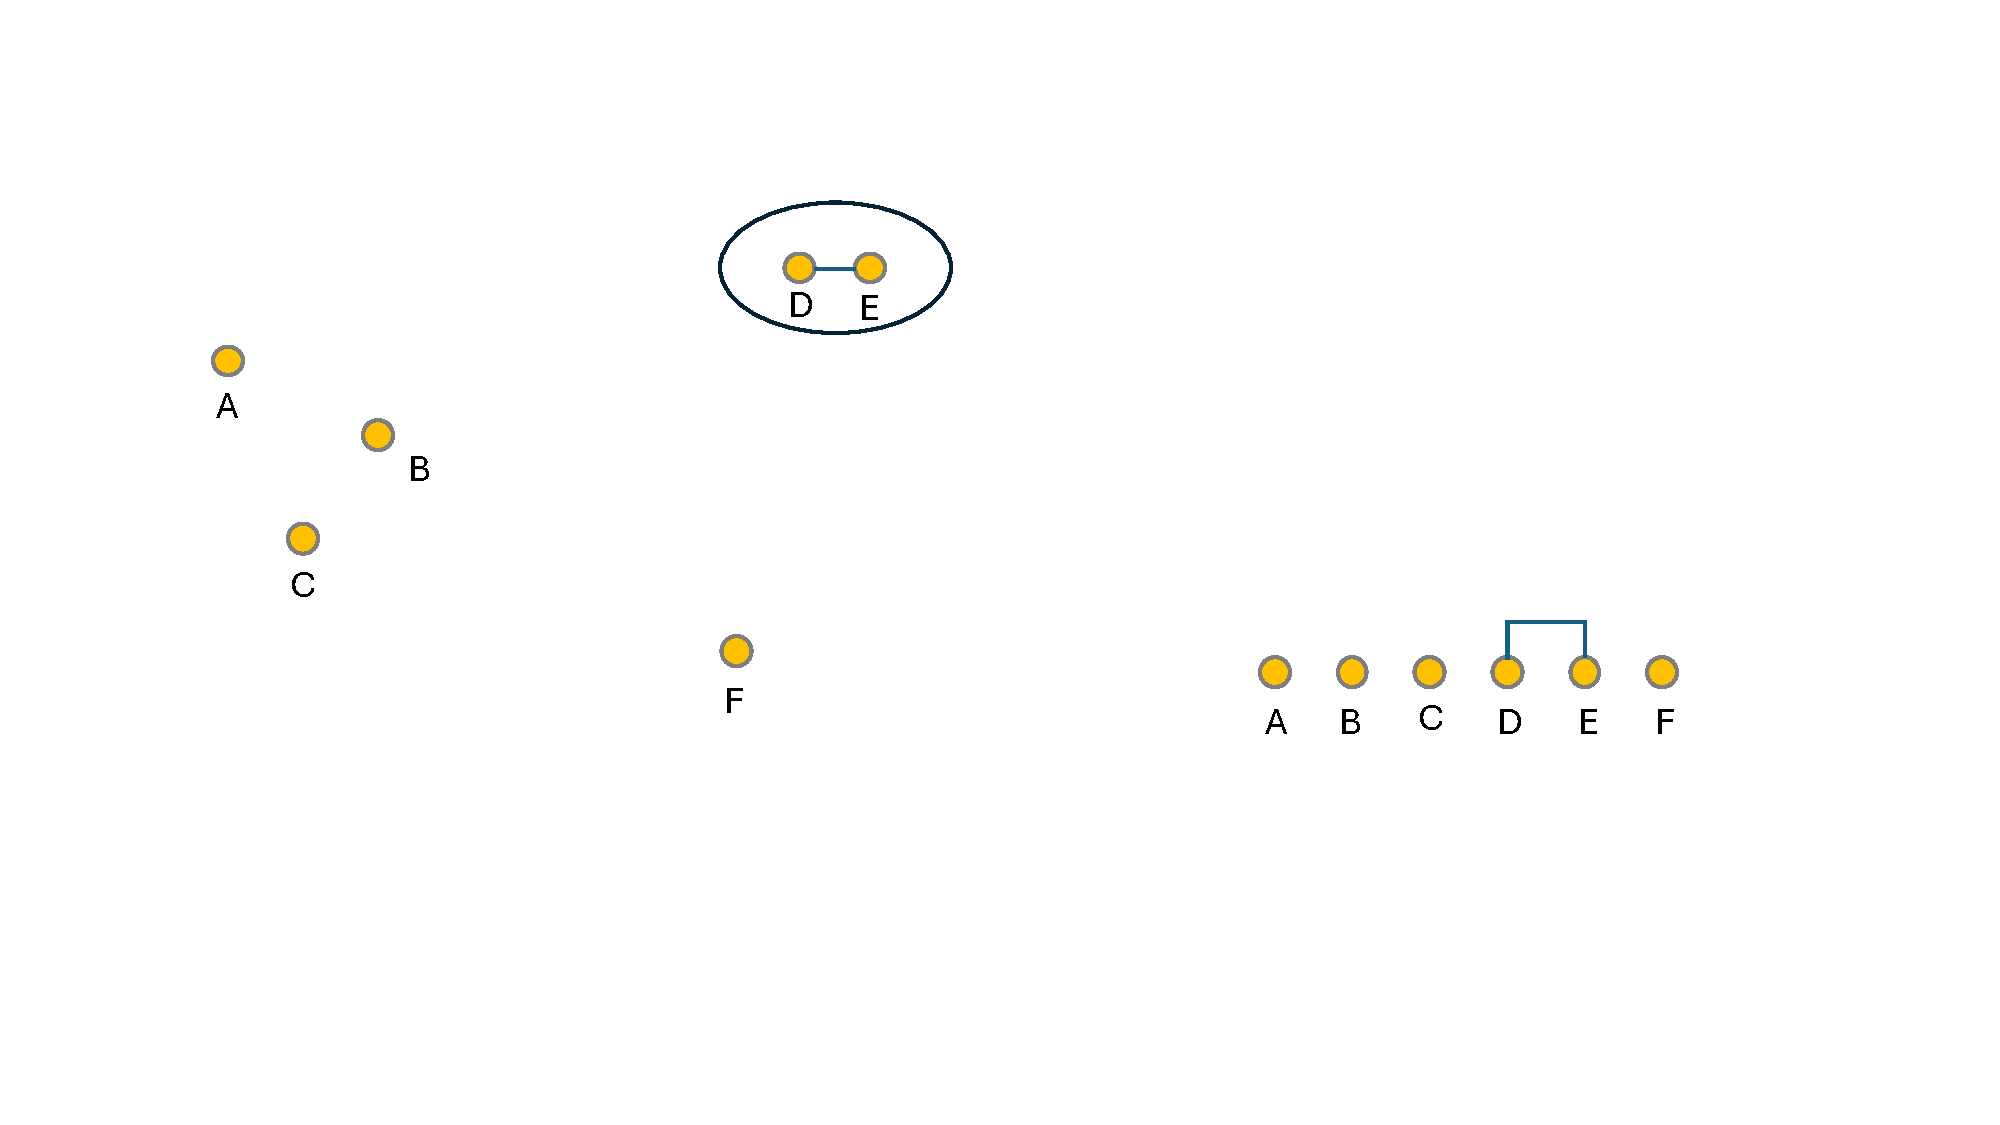
\includegraphics[width=0.8\textwidth]{figures/ch2}
  \end{center}
  Les deux points les plus proches sont fusionnés et forment le premier cluster.
\end{frame}

\begin{frame}
  \frametitle{Clustering hiérarchique -- Principe}
  \begin{center}
    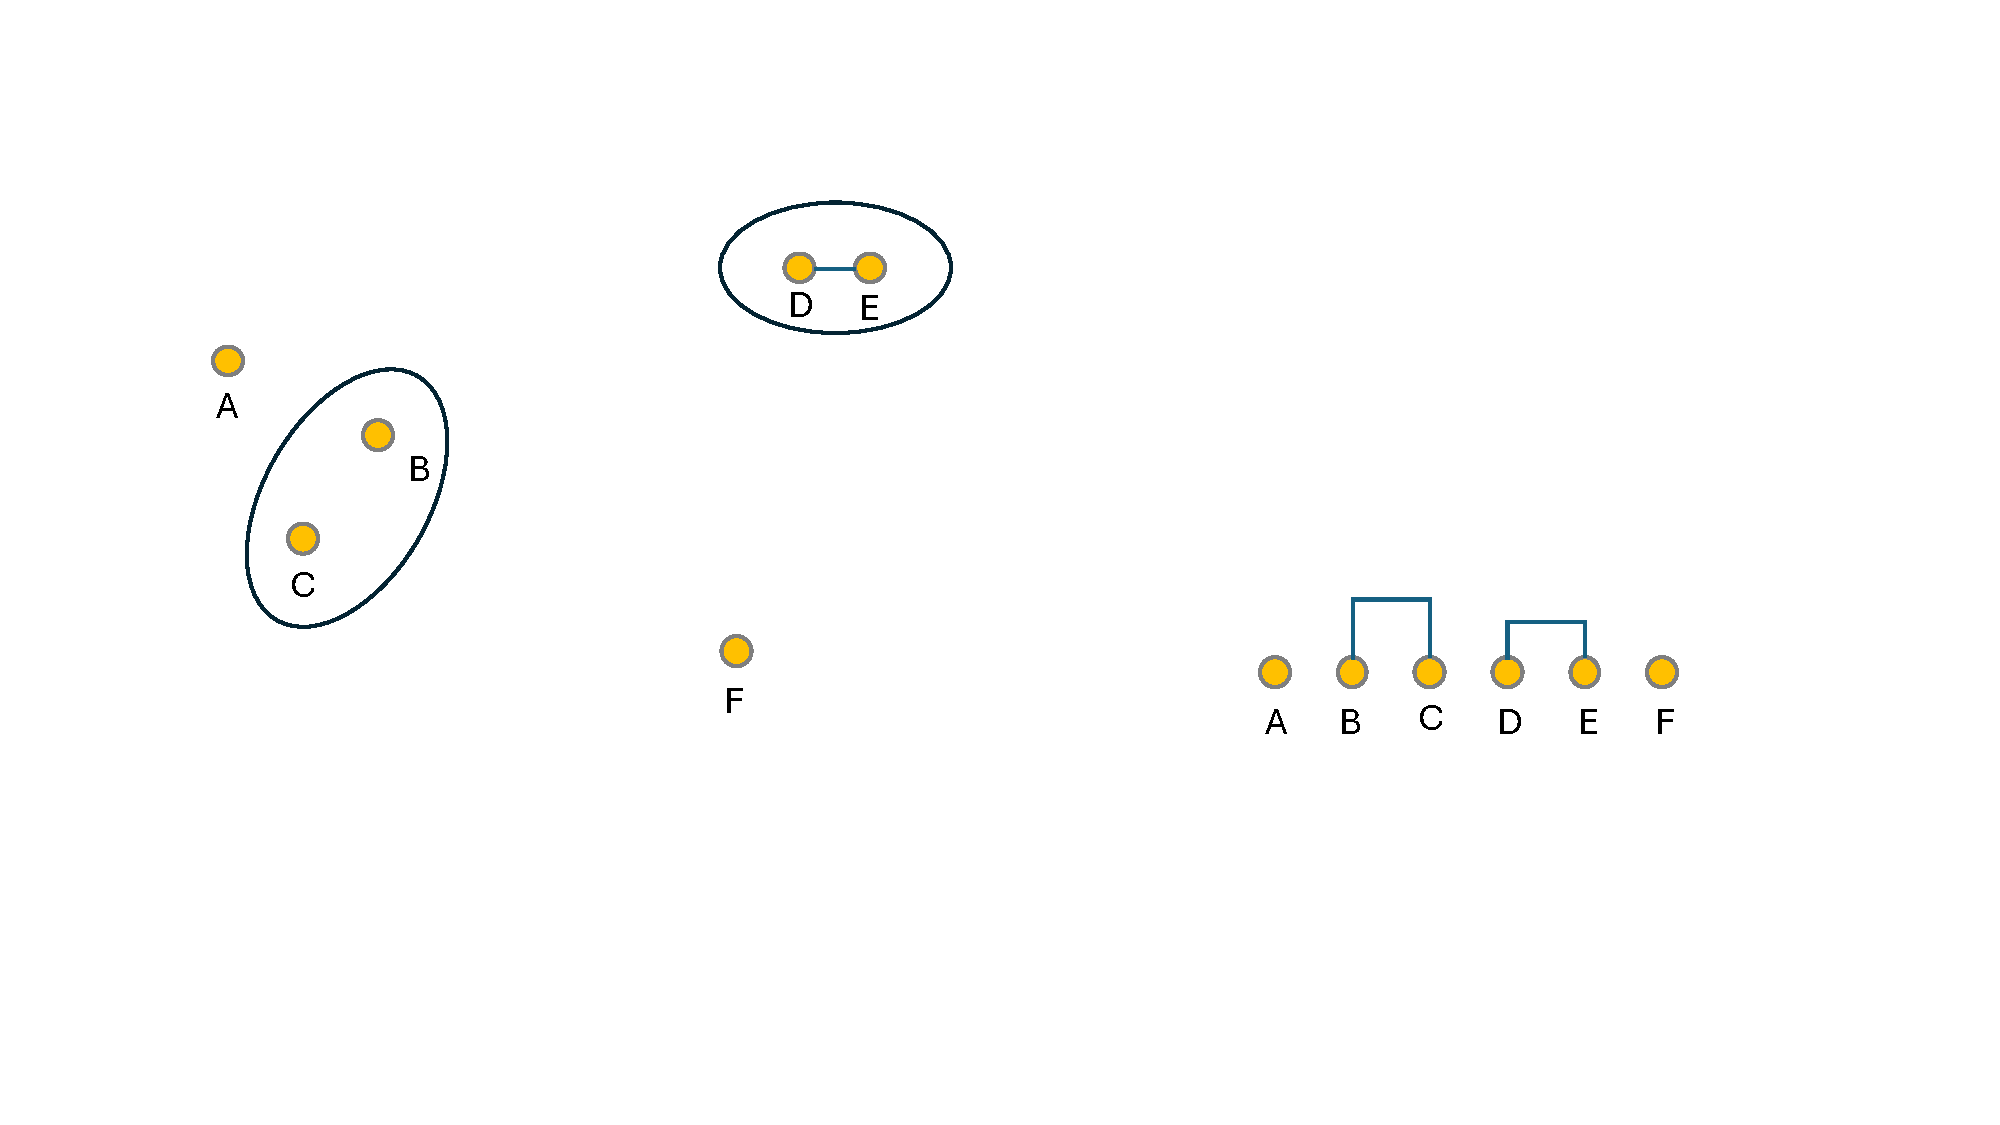
\includegraphics[width=0.8\textwidth]{figures/ch3}
  \end{center}
  Ensuite, les points ou clusters les plus proches sont fusionnés pour former un nouveau cluster.
\end{frame}

\begin{frame}
  \frametitle{Clustering hiérarchique -- Principe}
  \begin{center}
    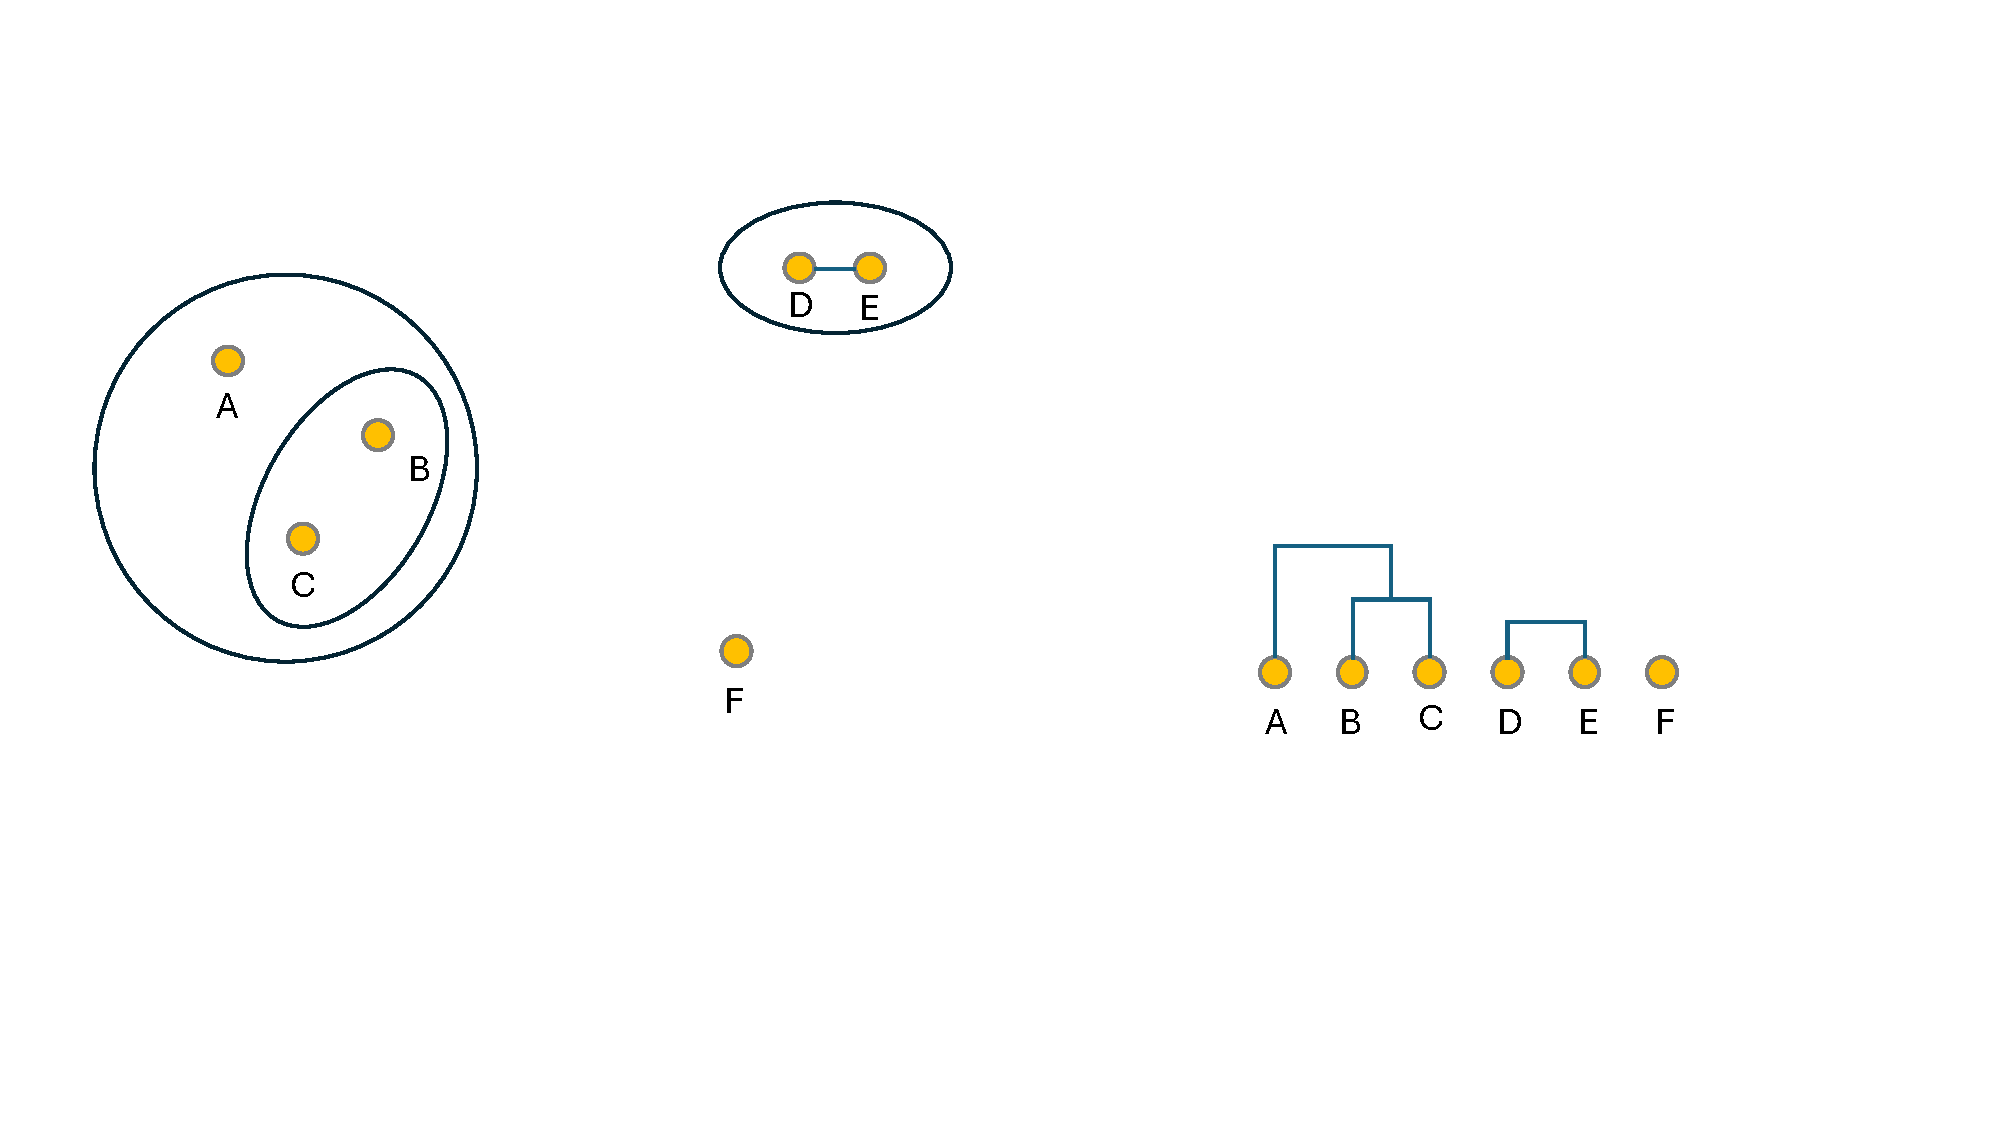
\includegraphics[width=0.8\textwidth]{figures/ch4}
  \end{center}
  Un dendrogramme est construit afin de garder la trace des fusions successives.
\end{frame}

\begin{frame}
  \frametitle{Clustering hiérarchique -- Principe}
  \begin{center}
    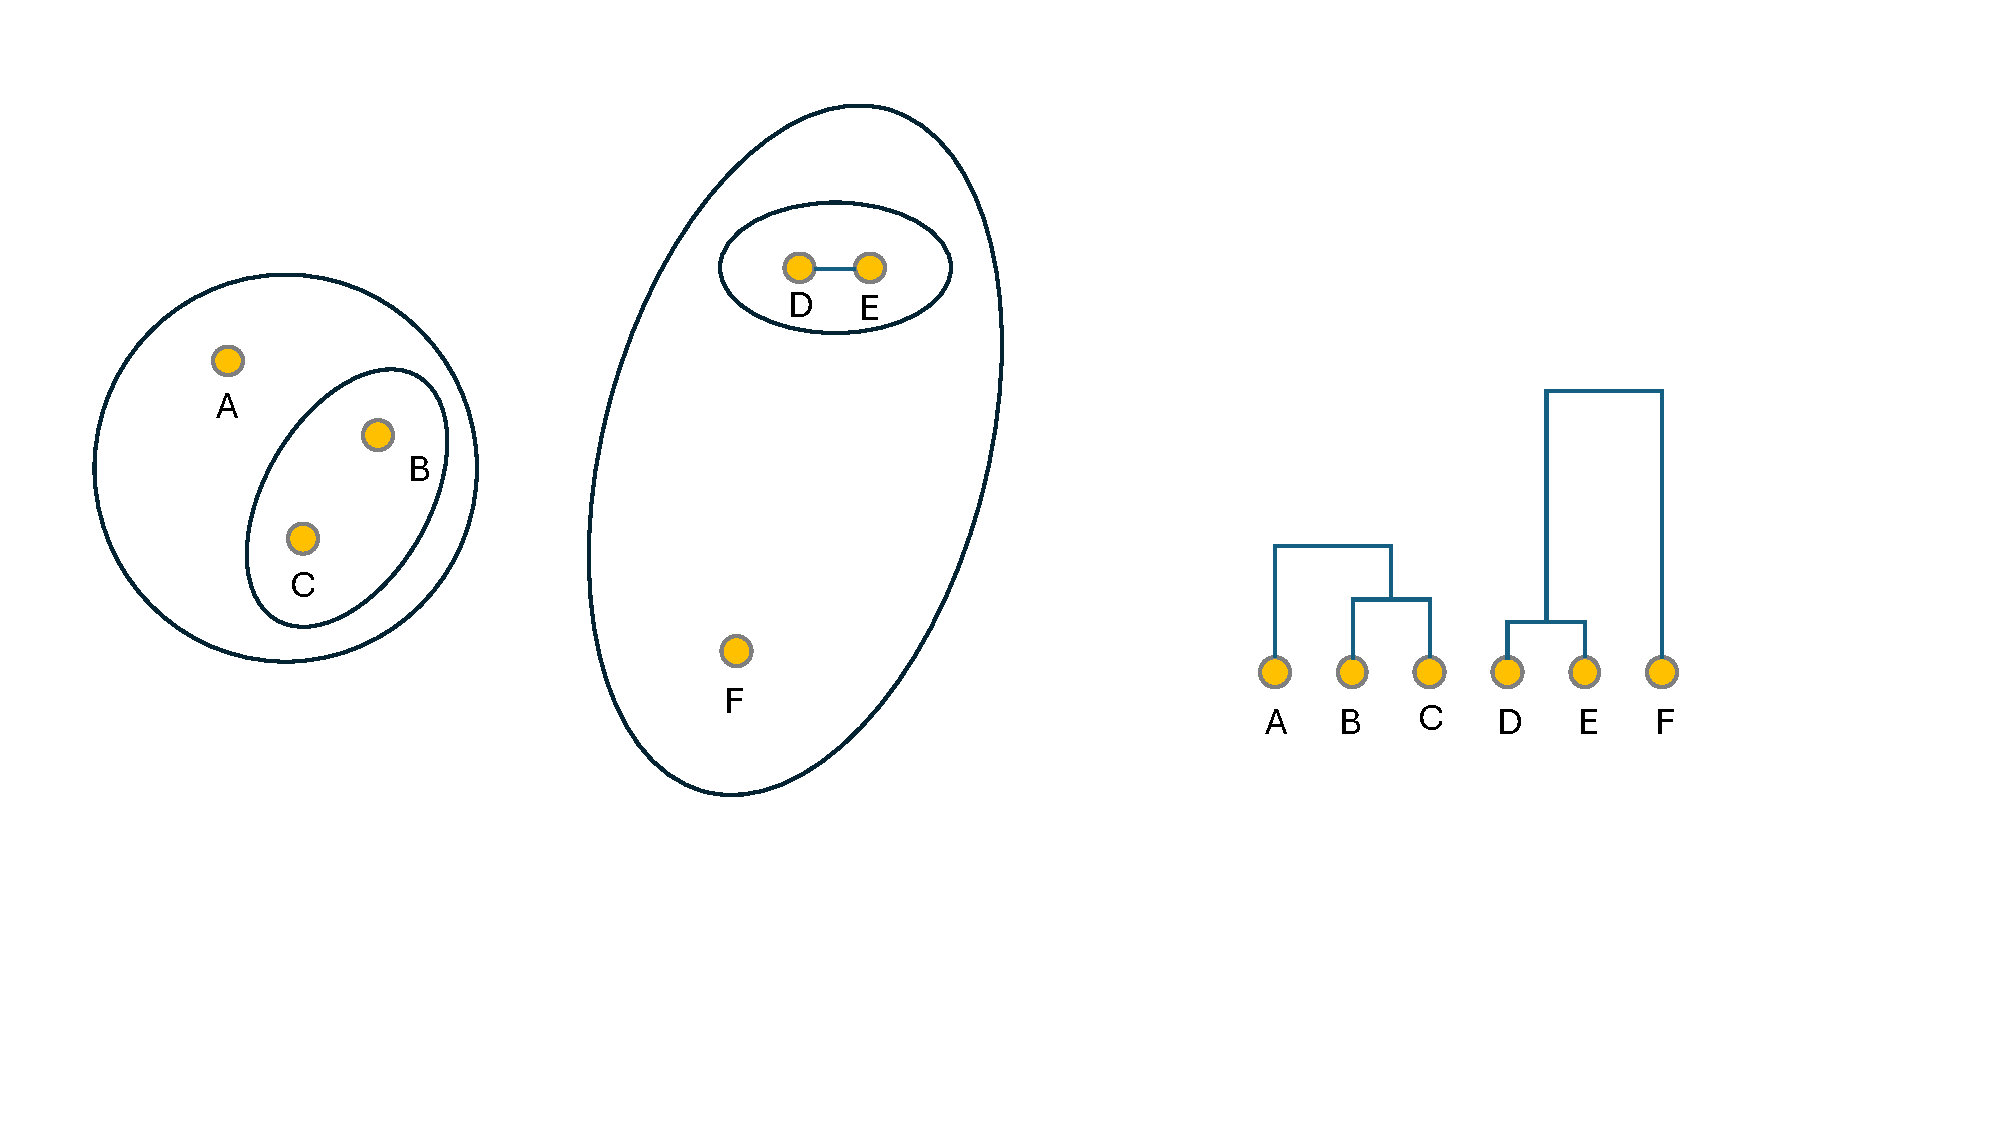
\includegraphics[width=0.8\textwidth]{figures/ch5}
  \end{center}
  La hauteur de chaque fusion correspond à la distance à laquelle cette fusion a lieu.
\end{frame}

\begin{frame}
  \frametitle{Clustering hiérarchique -- Principe}
  \begin{center}
    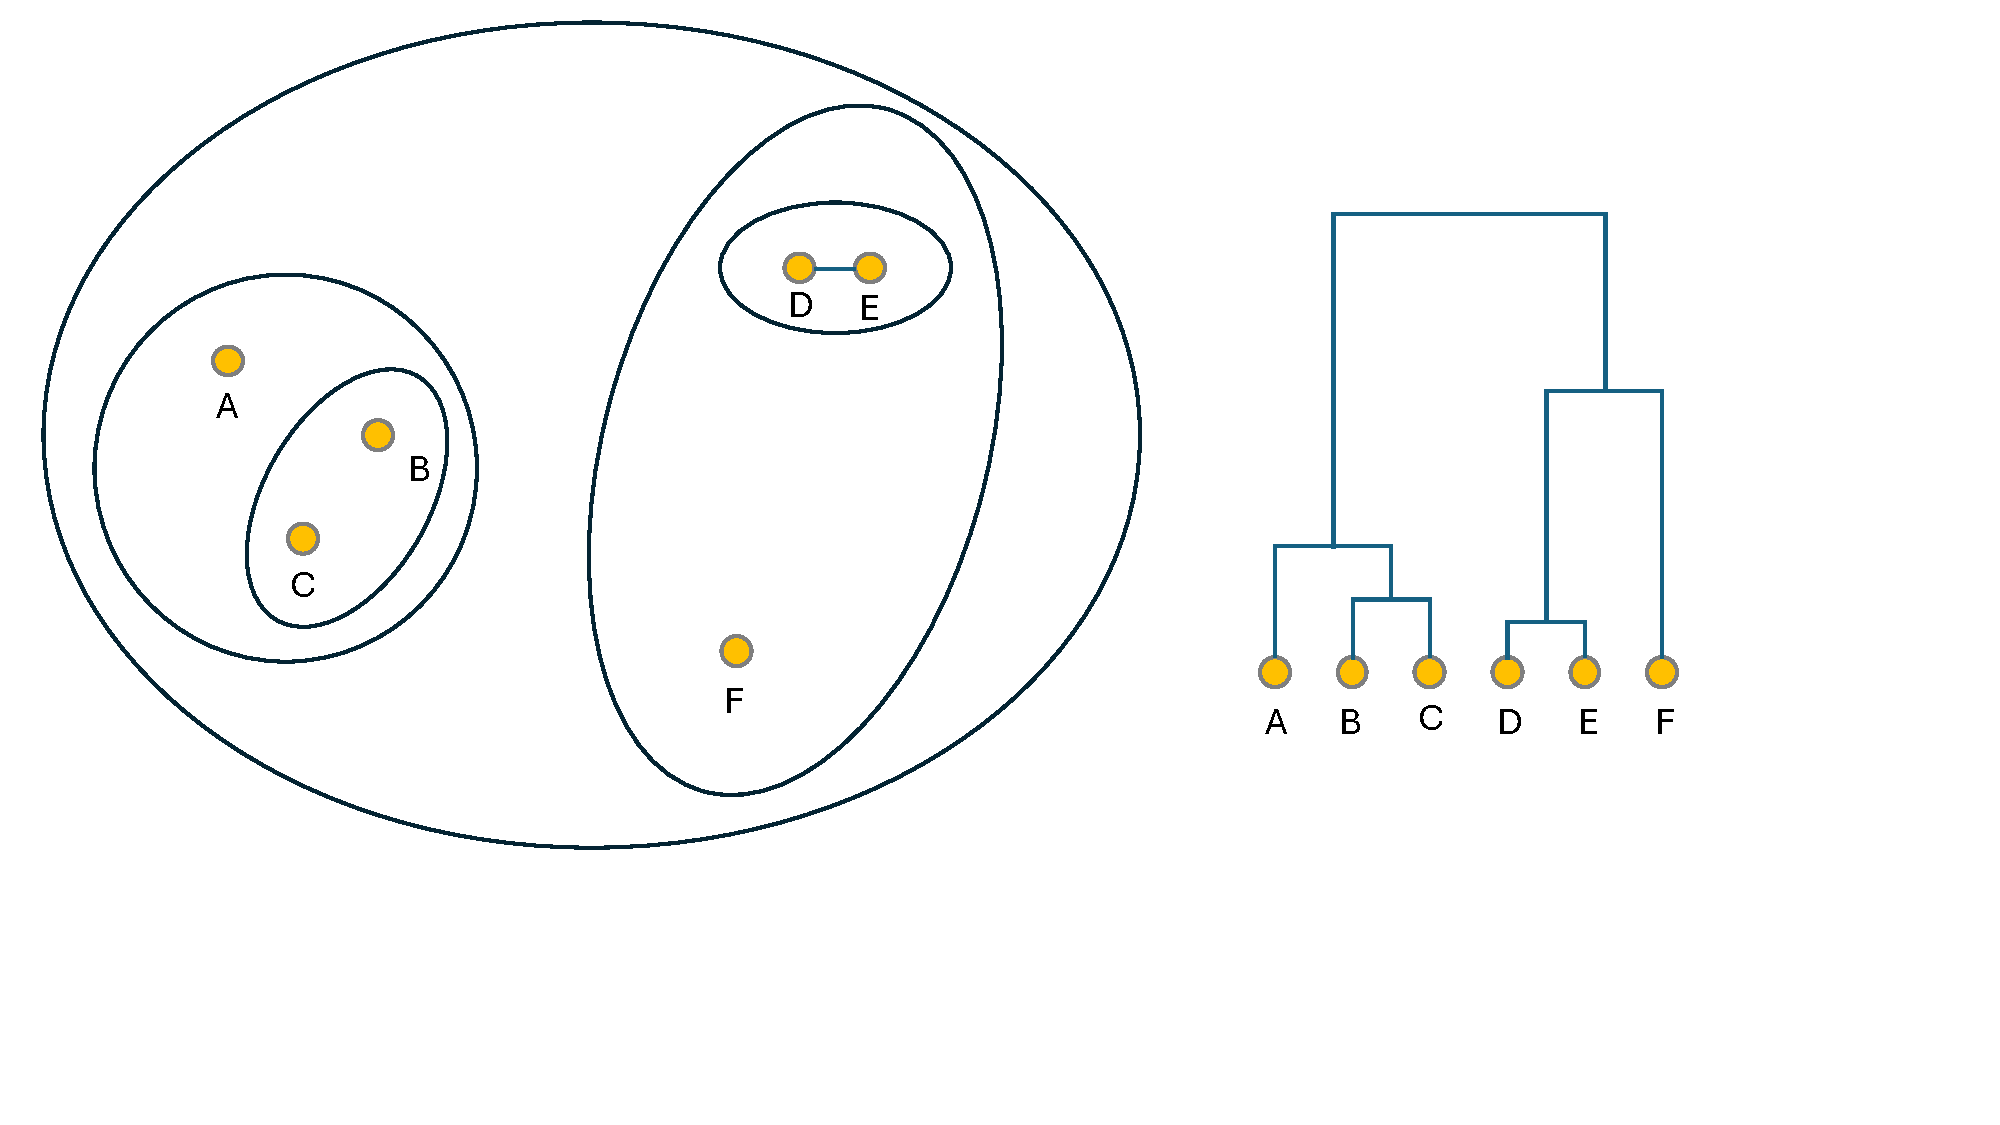
\includegraphics[width=0.8\textwidth]{figures/ch6}
  \end{center}
  Le clustering s'arrête lorsque tous les points appartiennent à un unique cluster global.
\end{frame}

\begin{frame}
  \frametitle{Clustering hiérarchique -- Deux ingrédients}
  \begin{itemize}
    \item Distance entre les points :
    \begin{itemize}
      \item Rappel : chaque échantillon $\xvec_i$ correspond à un point dans l'espace des caractéristiques.
      \item Comment calculer la distance entre deux points, c'est-à-dire entre deux échantillons ?
    \end{itemize}
    \item Distance entre les clusters :
    \begin{itemize}
      \item Option 1 : représenter chaque cluster par un prototype et calculer une distance entre points.
      \item Option 2 : calculer une agrégation des distances entre points.
    \end{itemize}
  \end{itemize}
\end{frame}

\begin{frame}{Clustering hiérarchique : distances entre points}
\begin{itemize}
  \item On considère ici deux points $\xvec$ et $\yvec$ ; les indices désignent les composantes des vecteurs.
  \item \textbf{Distance euclidienne} $d(\xvec,\yvec) = \sqrt{\sum_i (\xvec_i-\yvec_i)^2}$
  \item \textbf{Distance de Manhattan} $d(\xvec,\yvec) = \sum_i |\xvec_i-\yvec_i|$
  \item \textbf{Distance cosinus} $d(\xvec,\yvec) = 1 - \frac{\xvec^\top \yvec}{\|\xvec\|\|\yvec\|}$
  \item \textbf{Distance de corrélation} $d(\xvec,\yvec) = 1 - \mathrm{corr}(\xvec,\yvec)$
%  \item \textbf{Distance de Mahalanobis} $d(\xvec,\yvec) = \sqrt{(\xvec-\yvec)^\top \Sigma^{-1}(\xvec-\yvec)}$
\end{itemize}
\end{frame}



\begin{frame}
  \frametitle{Fonctions de lien}
  \begin{itemize}
  \item \red{Fonction de lien} \textcolor{gray!70}{(linkage)} : distance entre deux clusters
    \begin{itemize}
    \item \red{Lien simple} \textcolor{gray!70}{(single linkage)}
      \[ d_{\text{simple}}(\cset_k, \cset_l) = \min_{(\uvec, \vvec) \in \cset_k \times \cset_l } d(\uvec, \vvec).
      \]
      \pause
    \item \red{Lien complet} \textcolor{gray!70}{(complete linkage)}
      \[
        d_{\text{complet}}(\cset_k, \cset_l) = \max_{(\uvec, \vvec) \in \cset_k \times \cset_l} d(\uvec, \vvec).
      \]
      \pause
    \item \red{Lien moyen} \textcolor{gray!70}{(average linkage)} ou UPGMA \textcolor{gray!70}{(Unweighted Paired Group Method with Arithmetic mean)}
      \[
        d_{\text{moyen}}(\cset_k, \cset_l) = \frac1{\lvert \cset_k \rvert} 
        \frac1{\lvert \cset_l \rvert}
        \sum_{\uvec \in \cset_k}\sum_{\vvec \in \cset_l} d(\uvec, \vvec).
      \]
    \end{itemize}
  \end{itemize}
\end{frame}

\begin{frame}[t]
  \frametitle{Fonctions de lien}
  \begin{itemize}
  \item \red{Fonction de lien} \textcolor{gray!70}{(linkage)} : distance entre deux clusters
    \begin{itemize}
    \item \red{Lien centroïdal} \textcolor{gray!70}{(centroid linkage)}
      \[
        d_{\text{centroidal}}(\cset_k, \cset_l) = d \left (\frac1{\lvert \cset_k \rvert} 
          \sum_{\uvec \in \cset_k} \uvec, 
          \frac1{\lvert \cset_l \rvert} \sum_{\vvec \in \cset_l} \vvec \right) = 
        d(\muvec_k, \muvec_l).
      \]
    \end{itemize}
  \end{itemize}
\end{frame}










% -------------------------------------------------------------------------
\begin{frame}
  \begin{center}
    \large{3. Algorithme des k-moyennes}
  \end{center}
\end{frame}

\begin{frame}
  \frametitle{Variance intra-cluster}
  \begin{itemize}
  \item \red{Variance intra-cluster}
    \[
            \text{Var}_\text{in}(\cset) = \frac1{\lvert \cset \rvert} \sum_{\xvec \in \cset}
      \ltwonorm{\xvec - \muvec}^2.
    \]
  \item Minimiser la variance intra-cluster : créer des clusters \blue{homogènes}
  \end{itemize}
\end{frame}

\begin{frame}
  \frametitle{Algorithme de Lloyd}
  \begin{itemize}
  \item \blue{Initialisation :} choisir les $\muvec_1, \muvec_2, \ldots, \muvec_K$ parmi les données. 
  \item \blue{Affecter} chaque observation $\xvec \in \dset$ au centroïde dont elle est le plus proche :
    \begin{equation*}
      k(\xvec^i) = \argmin_{k=1, \ldots, K}\ltwonorm{\xvec^i - \muvec_k}^2
    \end{equation*}
  \item \blue{Recalculer} les centroïdes $\muvec_k$. 
  \item \blue{Répéter} jusqu'à ce que les affectations ne changent plus. 
  \end{itemize}
\end{frame}

\begin{frame}
  \frametitle{Algorithme de Lloyd}
  \begin{itemize}
  \item \blue{Avantages :}
    \begin{itemize}
    \item Converge rapidement en pratique
    \end{itemize}
    \pause
  \item \blue{Inconvénients :}
    \begin{itemize}
    \item Nécessité de fixer $K$ 
    \item Approche \blue{gloutonne} : pas de garantie de minimum global
    \item \blue{Stochasticité} : dépend de l'initialisation \pause $\rightarrow$ k-means++ 
    \item Clusters nécessairement \blue{convexes} \pause $\rightarrow$ kernel k-means
    \end{itemize}
  \end{itemize}
\end{frame}



% -------------------------------------------------------------------------


% -------------------------------------------------------------------------

\begin{frame}
  \begin{center}
    \large{4. DBSCAN}
  \end{center}
\end{frame}

\begin{frame}
  \frametitle{DBSCAN: Motivation}
  \begin{center}
    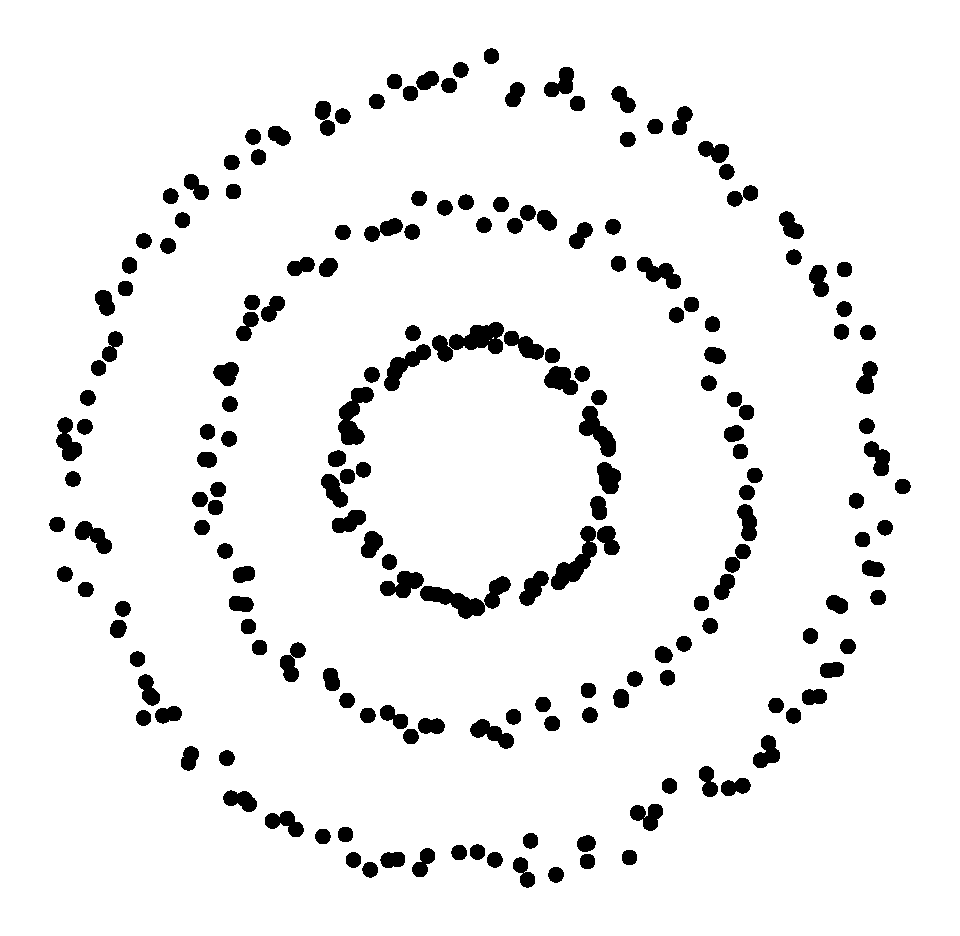
\includegraphics[width=.3\textwidth]{figures/dbscan_pb}%
    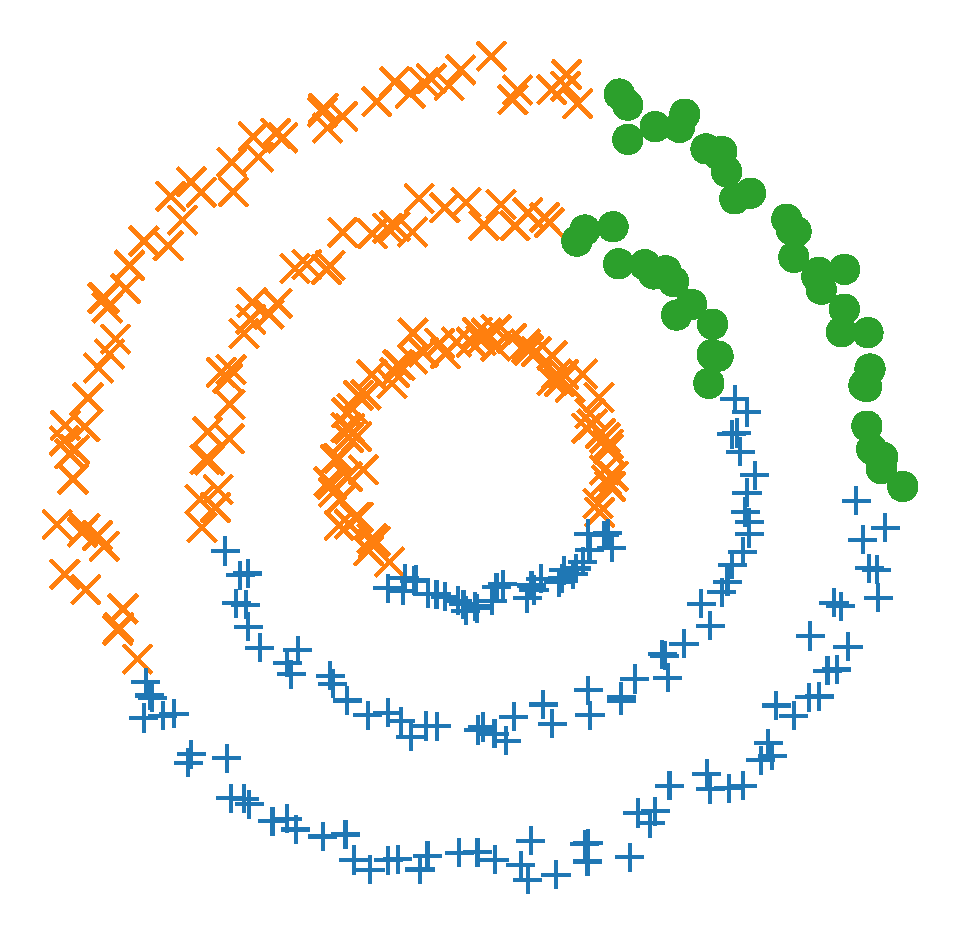
\includegraphics[width=.3\textwidth]{figures/hierarchical_sol}% 
    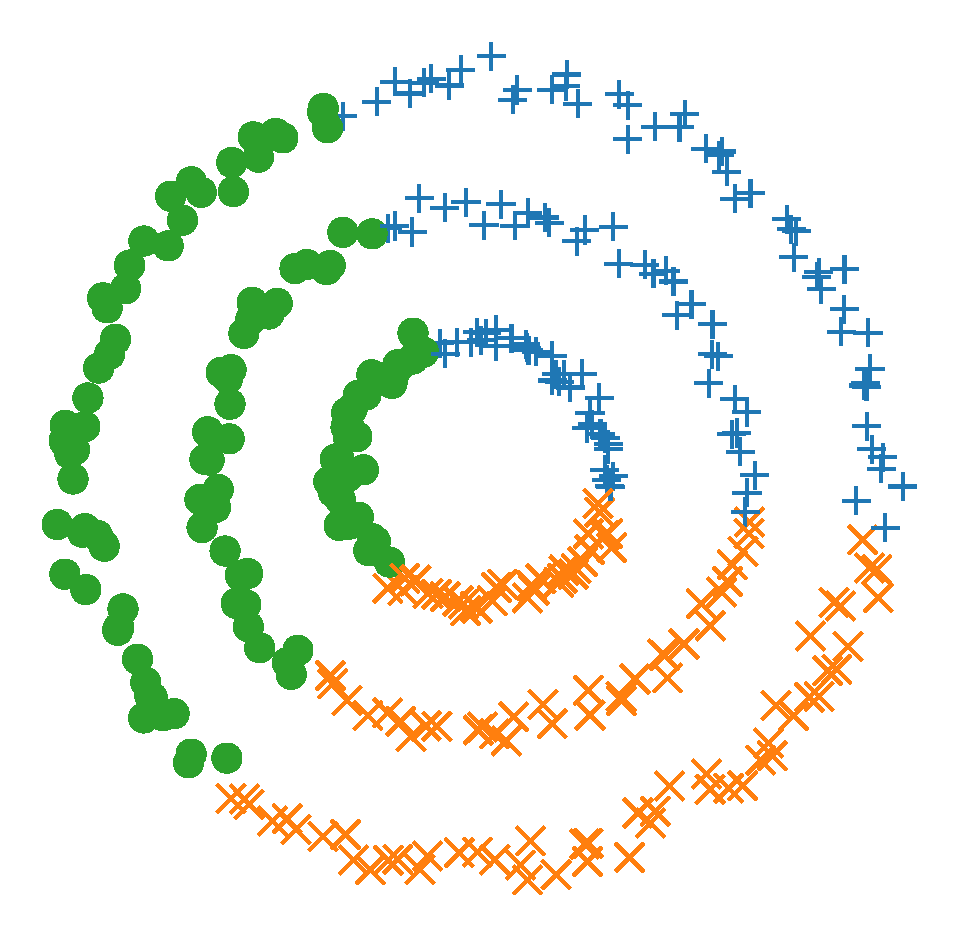
\includegraphics[width=.3\textwidth]{figures/kmeans_sol}
    
    {\small Nuage de points -- clustering hiérarchique -- clustering kmeans}
  \end{center}
  \begin{itemize}
  \item Idée : utiliser la \blue{densité}
  \end{itemize}
\end{frame}


% \begin{frame}
%   \frametitle{DBSCAN}
%   \begin{itemize}
%   \item Idée : itérer \blue{de proche en proche} par des \blue{voisinages} (boules) de rayon $\varepsilon$
%   \item On définit deux paramètres : (1) un rayon $\varepsilon$ et (2) un number minimal de points $n_{min}$. On définit alors : 
%   \begin{itemize}
%     \item Point cœur (core point) : un point ayant au moins $n_{min}$ voisins dans un rayon $\varepsilon$.
%     \item Point frontière (border point) : moins de $n_{min}$ dans son voisinage, mais il est proche d’un point coeur.
%     \item Point bruit (noise / outlier) : les points isolés, considérés comme du bruit .
%   \end{itemize}
%   \item Etapes de l'algorithmes : 
%   \begin{itemize}
%     \item On trouve d'abord les points coeurs. 
%     \item Ensuite, on construit les composantes connexes en reliant entre eux les points coeurs voisins : chaque composante constitue un cluster. 
%     \item Ensuite on assigne chaque point frontière à une composante connexe. 
%     \item On n'assigne pas les points bruit. 
%   \end{itemize}
%   % \begin{center}
%   %   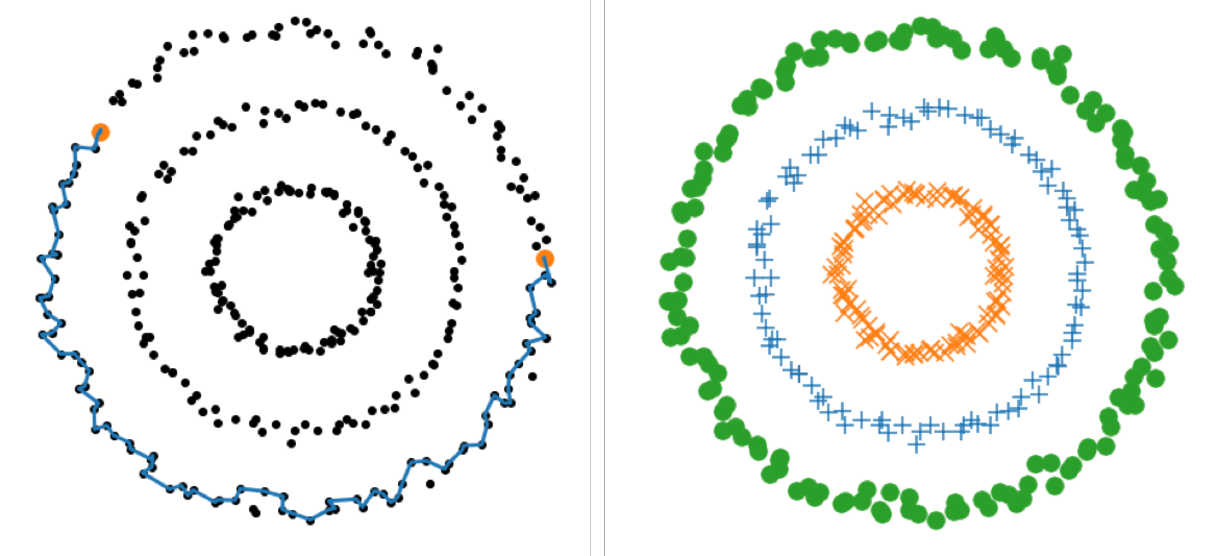
\includegraphics[width=.6\textwidth]{figures/dbscan}
%   % \end{center}
% \end{frame}

\begin{frame}
  \frametitle{DBSCAN}
  \begin{itemize}
  \item Idée : itérer \blue{de proche en proche} par des \blue{voisinages} (boules) de rayon $\varepsilon$
  \item On définit deux paramètres : 
  \begin{enumerate}
    \item un rayon $\varepsilon$ 
    \item un nombre minimal de points $n_{min}$. 
  \end{enumerate}
  \item On définit alors : 
  \begin{itemize}
    \item Point cœur (core point) : un point ayant au moins $n_{min}$ voisins dans un rayon $\varepsilon$.
    \item Point frontière (border point) : moins de $n_{min}$ dans son voisinage, mais il est proche d’un point coeur.
    \item Point bruit (noise / outlier) : les points isolés, considérés comme du bruit .
  \end{itemize}
\end{itemize}
\end{frame}

\begin{frame}
  \frametitle{DBSCAN}
  \begin{itemize}
  \item Etapes de l'algorithme : 
  \begin{itemize}
    \item On trouve d'abord les points coeurs. 
    \item Ensuite, on construit les composantes connexes en reliant entre eux les points coeurs voisins : chaque composante constitue un cluster. 
    \item Ensuite on assigne chaque point frontière à une composante connexe. 
    \item On n'assigne pas les points bruit. 
  \end{itemize}
  \end{itemize}
  \begin{center}
    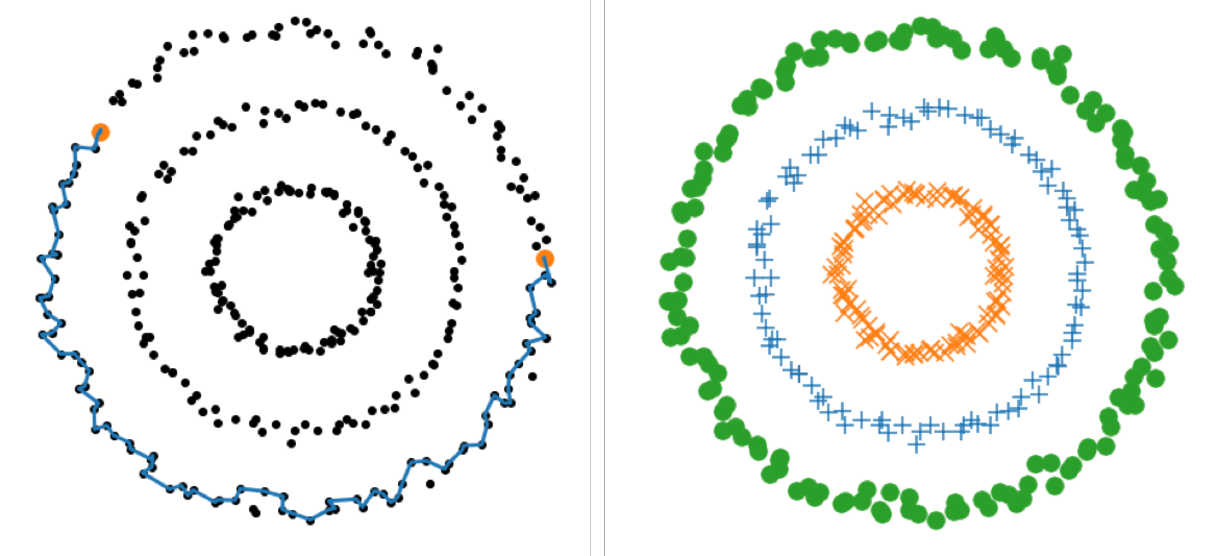
\includegraphics[width=.6\textwidth]{figures/dbscan}
  \end{center}
\end{frame}

\begin{frame}
  \frametitle{DBSCAN : avantages et inconvénients}
  \begin{itemize}
  \item \blue{Avantages :}
    \begin{itemize}
    \item n'impose pas de forme particulière
    \item simple, pas de définition du nombre de clusters
    \item robustesse aux données aberrantes
    \end{itemize}
  \pause
  \item \blue{Inconvénients :}
    \begin{itemize}
    \item ne sait pas gérer des écarts
    \item peu de résultats théoriques
    \item pas applicable en très haute dimension 
    \end{itemize}
    \pause
    \item \red{HDBSCAN} est une extension de DBSCAN qui résoud une grande partie des problèmes de DBSCAN. 
  \end{itemize}
\end{frame}


% -------------------------------------------------------------------------
\begin{frame}
  \frametitle{Clustering : conclusion}
  \begin{itemize}
    \item Le clustering désigne le partitionnement d'un jeu de données $\{\xvec_i\}_{i=1..N}$ en groupes.
    \item Il existe de nombreuses mesures de qualité pour évaluer un clustering :
    \begin{itemize}
      \item Mesures géométriques et séparabilité
      \item Robustesse
      \item Comparaison à une vérité terrain partielle
    \end{itemize}
    \item Algorithmes :
    \begin{itemize}
      \item Clustering hiérarchique : utile pour l'exploration
      \item k-means : méthode la plus populaire, mais il faut fixer le nombre de clusters
      \item DBSCAN / HDBSCAN : méthodes largement utilisées
    \end{itemize}
  \end{itemize}
\end{frame}

\begin{frame}
  \frametitle{Clustering : limites}
  \begin{itemize}
    \item Il n'existe pas de méthode générale permettant d'affirmer qu'un clustering « a du sens », sauf par comparaison, systématique ou anecdotique, avec une vérité terrain.
    \item Structure de corrélation :
    \begin{itemize}
      \item Des données fortement corrélées vont dominer les distances : $d(\xvec, \yvec) = \sqrt{\sum_i(x_i -  y_i)^2}$
      \item Utiliser une ACP pour décorréler les données ne résout pas ce problème, sauf si les composantes principales sont normalisées par rapport à leur variance, c'est-à-dire par whitening. Mais dans ce cas, on augmente aussi le bruit.
    \end{itemize}
    \item Il n'existe pas vraiment d'approche « non supervisée » :
    \begin{itemize}
      \item Nous choisissons les caractéristiques
      \item Nous choisissons les méthodes, les distances et les hyperparamètres
    \end{itemize}
  \end{itemize}
\end{frame}

\begin{frame}
  \frametitle{Clustering : un problème mal posé}
  \begin{center}
    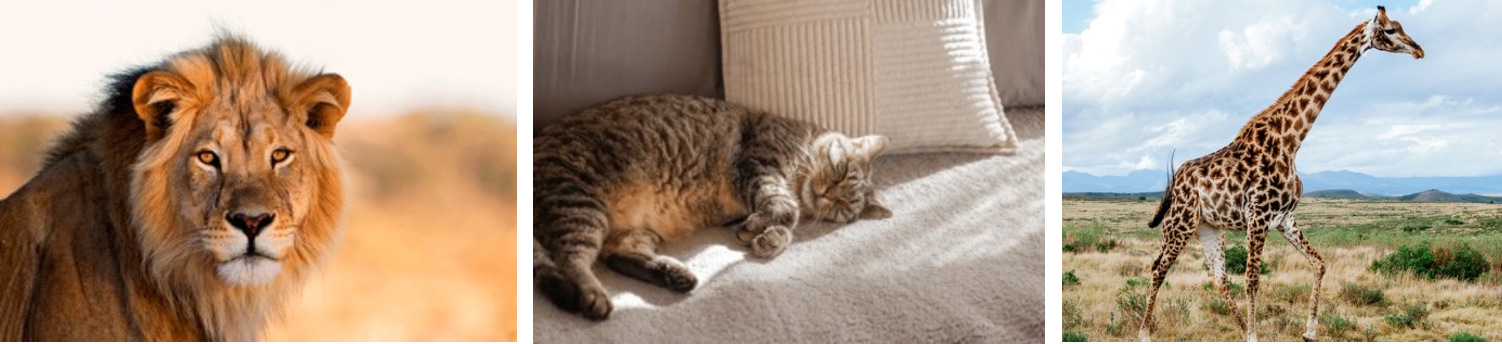
\includegraphics[width=0.9\textwidth]{figures/clustering_animals}
  \end{center}
  Comment définir deux groupes pour ces images ?
\end{frame}


% -------------------------------------------------------------------------
\begin{frame}
\frametitle{Conclusion générale - avant de commencer}
\begin{itemize}
\item Spécification du problème : 
\begin{itemize}
  \item supervisé ou non-supervisé ? 
  \item régression ou classification ? 
\end{itemize}
\item Quantification pour la mise en place:
\begin{itemize}
  \item combien de descripteurs ($p$) ? 
  \item combien d'échantillons annotés ($n$) ? 
  \item combien d'échantillons non-annotés ?
\end{itemize}
\end{itemize}
\end{frame}

\begin{frame}
\frametitle{Conclusion générale - avant de commencer}
\begin{itemize}
  \item Exigences supplémentaires : 
  \begin{itemize}
    \item interprétabilité des modèles
    \item robustesse 
    \item compromis sensibilité / précision
    \item biais et perturbations potentiels
  \end{itemize}
\end{itemize}
\end{frame}

\begin{frame}
\frametitle{Conclusion générale - méthodes non-supervisées}
\begin{itemize}
  \item Exploration graphique des données : 
  \begin{itemize}
    \item Réduction de dimensions (ACP, t-SNE)
    \item Clustering pour trouver des groupes
  \end{itemize}
  \item Le but est comprendre les distributions des données et éventuellement d'identifier des groupes. 
  \item Visualisation joue souvent un rôle clé pendant cette phase exploratoire.
\end{itemize}
\end{frame}

\begin{frame}
\frametitle{Conclusion générale - problèmes supervisés}
\begin{itemize}
  \item Si $n \gg p$ : 
  \begin{itemize}
    \item des méthodes classiques comme la $LDA$ ou la régression logistique peuvent s'appliquer. 
    \item Problème potentiel : corrélation des descripteurs. Solution possible : sélectionner les descripteurs, ou bien appliquer une $ACP$. 
    \item Tester l'effet d'une régularisation. 
  \end{itemize}
  \item Si $p > n$ (et même si $p \gg n$): 
  \begin{itemize}
    \item les $SVM$ ou les $RF$ sont préférables. 
    \item la régularisation se fait avec la norme $L_2$ des paramètres pour les $SVM$ et par ensembling pour les $RF$. 
  \end{itemize}
\end{itemize}
\end{frame}


\begin{frame}
  \frametitle{Références / page pub}
  \begin{itemize}
  \item \black{Introduction au Machine Learning}, Chloé-Agathe Azencott, Dunod InfoSup \\
    Version électronique (PDF) sans exercices disponible gratuitement sur  \textcolor{MyBlue}{\href{http://cazencott.info/dotclear/public/lectures/IntroML_Azencott.pdf}{http://cazencott.info [lien cliquable]}}\\
    (nouvelle édition en préparation)
  \item \black{Le Machine Learning avec scikit-learn}, Aurélien Géron, Dunod
    InfoSup
  \item Textes et vidéos sur \blue{OpenClassrooms :} \\
    {\footnotesize Textes accessibles librement ; vidéos accessibles avec un compte gratuit.}
    \begin{itemize} 
    \item \textcolor{MyBlue}{\href{https://openclassrooms.com/fr/paths/148-ingenieur-machine-learning\#path-tabs}{Parcours Ingénieur Machine Learning [lien cliquable]}}
     \item \textcolor{MyBlue}{\href{https://openclassrooms.com/fr/courses/6417031-objectif-ia-initiez-vous-a-lintelligence-artificielle}{Objectif IA (grand public)  [lien cliquable]}}
    \end{itemize}
  \end{itemize}
\end{frame}

\begin{frame}
  \frametitle{Ressources complémentaires}
  \begin{itemize}
  \item \blue{Sources de jeux de données}
    \begin{itemize}
    \item Kaggle \href{https://www.kaggle.com/}{[lien cliquable]}
    \item Le module \texttt{datasets} de \texttt{scikit-learn} \textcolor{MyBlue}{\href{https://sklearn.org/datasets/index.html}{[lien cliquable]}}
    \item Le UCI Machine Learning Repository \textcolor{MyBlue}{\href{https://archive.ics.uci.edu/ml/index.php}{[lien cliquable]}}
    \end{itemize}
  \item \blue{MOOC scikit-learn } \textcolor{MyBlue}{\href{https://inria.github.io/scikit-learn-mooc/}{[lien cliquable]}}
  \end{itemize}
\end{frame}

